\documentclass[man]{apa6}

\usepackage{amssymb,amsmath}
\usepackage{ifxetex,ifluatex}
\usepackage{fixltx2e} % provides \textsubscript
\ifnum 0\ifxetex 1\fi\ifluatex 1\fi=0 % if pdftex
  \usepackage[T1]{fontenc}
  \usepackage[utf8]{inputenc}
\else % if luatex or xelatex
  \ifxetex
    \usepackage{mathspec}
    \usepackage{xltxtra,xunicode}
  \else
    \usepackage{fontspec}
  \fi
  \defaultfontfeatures{Mapping=tex-text,Scale=MatchLowercase}
  \newcommand{\euro}{€}
\fi
% use upquote if available, for straight quotes in verbatim environments
\IfFileExists{upquote.sty}{\usepackage{upquote}}{}
% use microtype if available
\IfFileExists{microtype.sty}{\usepackage{microtype}}{}

% Table formatting
\usepackage{longtable, booktabs}
\usepackage{lscape}
% \usepackage[counterclockwise]{rotating}   % Landscape page setup for large tables
\usepackage{multirow}		% Table styling
\usepackage{tabularx}		% Control Column width
\usepackage[flushleft]{threeparttable}	% Allows for three part tables with a specified notes section
\usepackage{threeparttablex}            % Lets threeparttable work with longtable

% Create new environments so endfloat can handle them
% \newenvironment{ltable}
%   {\begin{landscape}\begin{center}\begin{threeparttable}}
%   {\end{threeparttable}\end{center}\end{landscape}}

\newenvironment{lltable}
  {\begin{landscape}\begin{center}\begin{ThreePartTable}}
  {\end{ThreePartTable}\end{center}\end{landscape}}

  \usepackage{ifthen} % Only add declarations when endfloat package is loaded
  \ifthenelse{\equal{\string man}{\string man}}{%
   \DeclareDelayedFloatFlavor{ThreePartTable}{table} % Make endfloat play with longtable
   % \DeclareDelayedFloatFlavor{ltable}{table} % Make endfloat play with lscape
   \DeclareDelayedFloatFlavor{lltable}{table} % Make endfloat play with lscape & longtable
  }{}%



% The following enables adjusting longtable caption width to table width
% Solution found at http://golatex.de/longtable-mit-caption-so-breit-wie-die-tabelle-t15767.html
\makeatletter
\newcommand\LastLTentrywidth{1em}
\newlength\longtablewidth
\setlength{\longtablewidth}{1in}
\newcommand\getlongtablewidth{%
 \begingroup
  \ifcsname LT@\roman{LT@tables}\endcsname
  \global\longtablewidth=0pt
  \renewcommand\LT@entry[2]{\global\advance\longtablewidth by ##2\relax\gdef\LastLTentrywidth{##2}}%
  \@nameuse{LT@\roman{LT@tables}}%
  \fi
\endgroup}


  \usepackage{graphicx}
  \makeatletter
  \def\maxwidth{\ifdim\Gin@nat@width>\linewidth\linewidth\else\Gin@nat@width\fi}
  \def\maxheight{\ifdim\Gin@nat@height>\textheight\textheight\else\Gin@nat@height\fi}
  \makeatother
  % Scale images if necessary, so that they will not overflow the page
  % margins by default, and it is still possible to overwrite the defaults
  % using explicit options in \includegraphics[width, height, ...]{}
  \setkeys{Gin}{width=\maxwidth,height=\maxheight,keepaspectratio}
\ifxetex
  \usepackage[setpagesize=false, % page size defined by xetex
              unicode=false, % unicode breaks when used with xetex
              xetex]{hyperref}
\else
  \usepackage[unicode=true]{hyperref}
\fi
\hypersetup{breaklinks=true,
            pdfauthor={},
            pdftitle={Assignment Statistics 5},
            colorlinks=true,
            citecolor=blue,
            urlcolor=blue,
            linkcolor=black,
            pdfborder={0 0 0}}
\urlstyle{same}  % don't use monospace font for urls

\setlength{\parindent}{0pt}
%\setlength{\parskip}{0pt plus 0pt minus 0pt}

\setlength{\emergencystretch}{3em}  % prevent overfull lines


% Manuscript styling
\captionsetup{font=singlespacing,justification=justified}
\usepackage{csquotes}
\usepackage{upgreek}



\usepackage{tikz} % Variable definition to generate author note

% fix for \tightlist problem in pandoc 1.14
\providecommand{\tightlist}{%
  \setlength{\itemsep}{0pt}\setlength{\parskip}{0pt}}

% Essential manuscript parts
  \title{Assignment Statistics 5}

  \shorttitle{Bbayesian hierarchical modeling}


  \author{Gustavo Villca Ponce\textsuperscript{1}, MohammadHossein Haqiqatkhah\textsuperscript{2}, Sigert Ariens\textsuperscript{3}, \& Bavo Kempens\textsuperscript{4}}

  % \def\affdep{{"", "", "", ""}}%
  % \def\affcity{{"", "", "", ""}}%

  \affiliation{
    \vspace{0.5cm}
          \textsuperscript{1} r0292033\\
          \textsuperscript{2} r0607671\\
          \textsuperscript{3} r0446864\\
          \textsuperscript{4} r0585283\\
          \textsuperscript{} Faculty of Psychology and Educational Sciences, KU Leuven.  }



      \keywords{\\

      \indent  1613
    }
  




\usepackage{amsthm}
\newtheorem{theorem}{Theorem}[section]
\newtheorem{lemma}{Lemma}[section]
\theoremstyle{definition}
\newtheorem{definition}{Definition}[section]
\newtheorem{corollary}{Corollary}[section]
\newtheorem{proposition}{Proposition}[section]
\theoremstyle{definition}
\newtheorem{example}{Example}[section]
\theoremstyle{definition}
\newtheorem{exercise}{Exercise}[section]
\theoremstyle{remark}
\newtheorem*{remark}{Remark}
\newtheorem*{solution}{Solution}
\begin{document}

\maketitle

\setcounter{secnumdepth}{0}



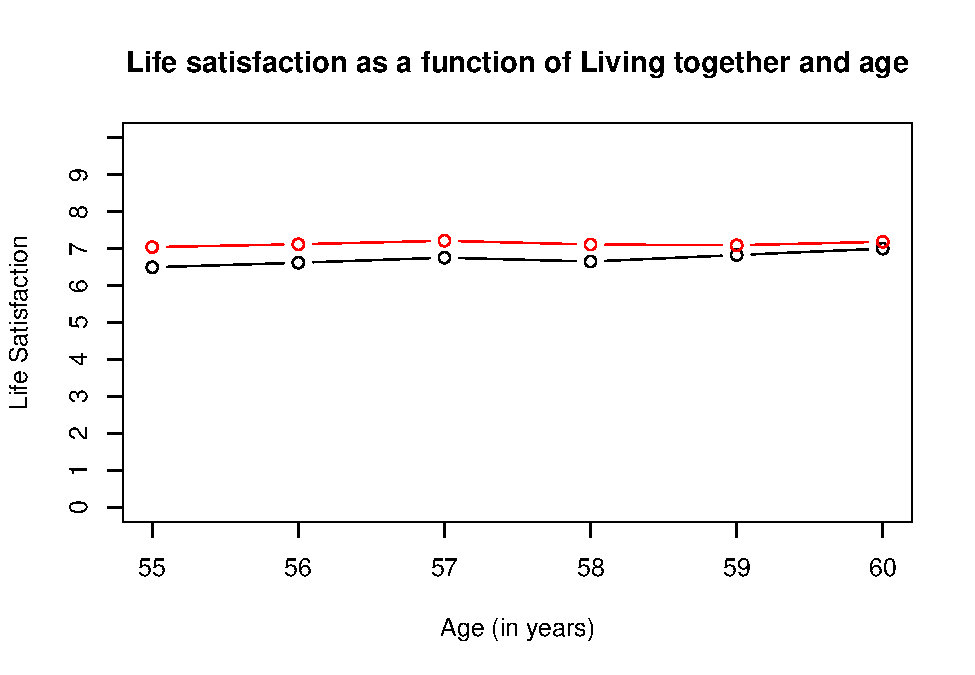
\includegraphics{Statistics-5-report-final-hours_files/figure-latex/exploratory plots-1.pdf}
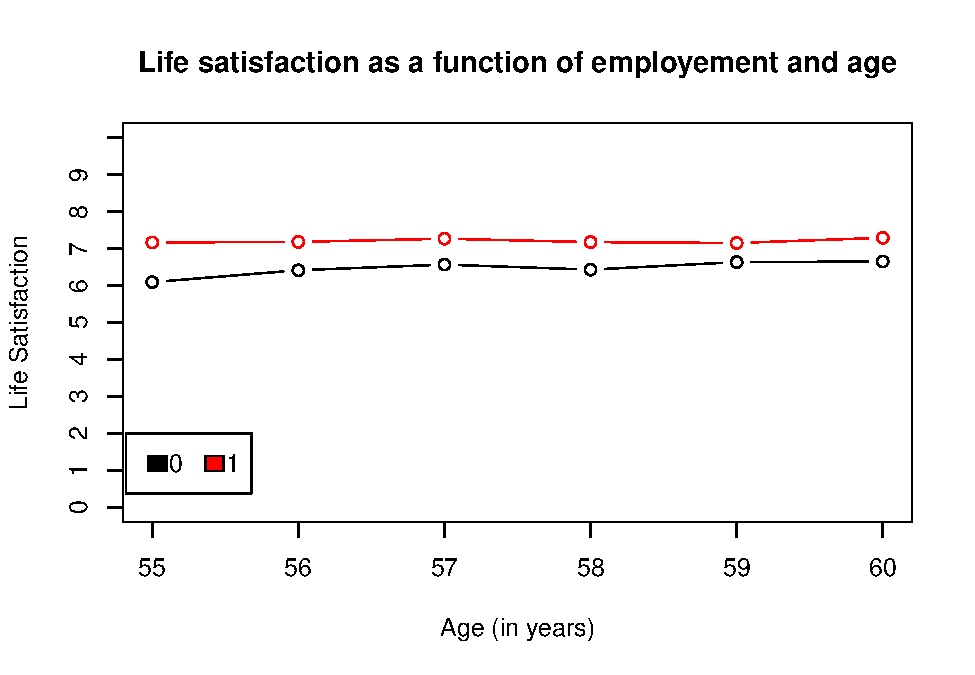
\includegraphics{Statistics-5-report-final-hours_files/figure-latex/exploratory plots-2.pdf}
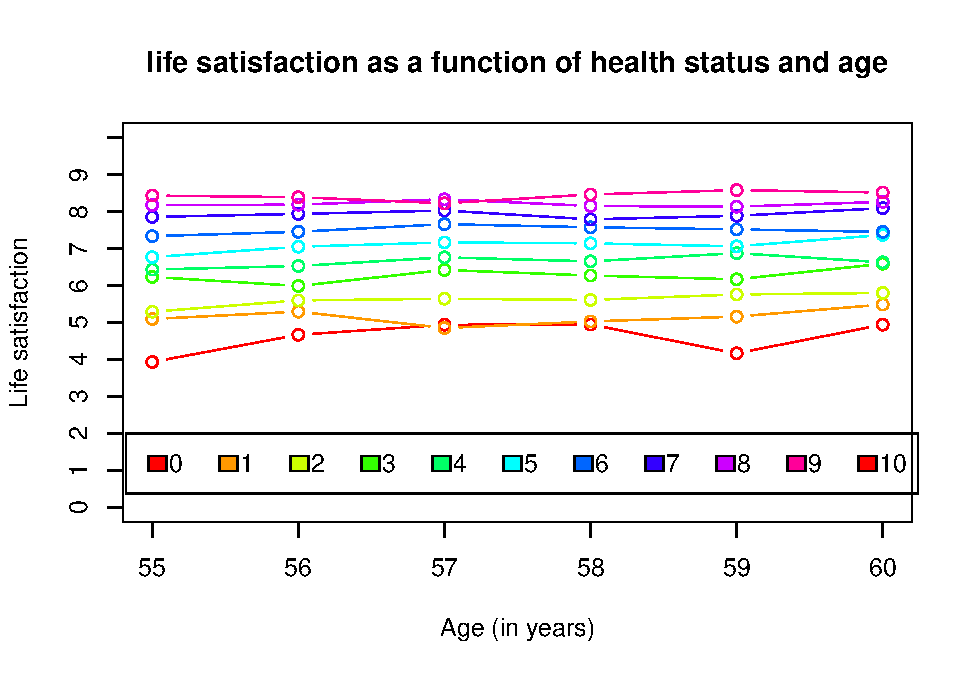
\includegraphics{Statistics-5-report-final-hours_files/figure-latex/exploratory plots-3.pdf}

\begin{lltable}
\begin{TableNotes}[para]
\textit{Note.} This table contains statistics pertaining to our replication of the original adjusted models.
\end{TableNotes}
\small{
\begin{longtable}{llllllllllll}\noalign{\getlongtablewidth\global\LTcapwidth=\longtablewidth}
\caption{\label{tab:tables of summaries}The first model}\\
\toprule
 & \multicolumn{1}{c}{Lower95} & \multicolumn{1}{c}{Median} & \multicolumn{1}{c}{Upper95} & \multicolumn{1}{c}{Mean} & \multicolumn{1}{c}{SD} & \multicolumn{1}{c}{Mode} & \multicolumn{1}{c}{MCerr} & \multicolumn{1}{c}{MC\%ofSD} & \multicolumn{1}{c}{SSeff} & \multicolumn{1}{c}{AC.1800} & \multicolumn{1}{c}{psrf}\\
\midrule
ss[1] & 0.54 & 0.60 & 0.66 & 0.60 & 0.03 & 0.60 & 0.00 & 2.20 & 2,000.00 & -0.01 & 1.00\\
ss[2] & 0.26 & 0.29 & 0.32 & 0.29 & 0.02 & 0.29 & 0.00 & 2.20 & 2,000.00 & 0.02 & 1.00\\
ss[3] & 0.42 & 0.57 & 0.72 & 0.57 & 0.08 & 0.56 & 0.00 & 2.20 & 2,000.00 & -0.02 & 1.00\\
cor12 & -0.02 & -0.01 & 0.01 & -0.01 & 0.01 & -0.01 & 0.00 & 2.10 & 2,363.00 & -0.01 & 1.00\\
cor13 & -0.36 & -0.21 & -0.08 & -0.22 & 0.08 & -0.20 & 0.00 & 2.20 & 2,000.00 & -0.02 & 1.00\\
cor23 & -0.15 & -0.07 & 0.00 & -0.07 & 0.04 & -0.06 & 0.00 & 2.20 & 2,000.00 & -0.03 & 1.00\\
betamu[1] & -0.39 & -0.30 & -0.21 & -0.30 & 0.05 & -0.29 & 0.00 & 2.00 & 2,551.00 & 0.00 & 1.00\\
betamu[2] & 0.30 & 0.35 & 0.40 & 0.35 & 0.03 & 0.35 & 0.00 & 2.20 & 2,106.00 & -0.02 & 1.00\\
betamu[3] & 0.11 & 0.19 & 0.27 & 0.19 & 0.04 & 0.19 & 0.00 & 2.20 & 2,060.00 & 0.01 & 1.00\\
betax[1] & 0.13 & 0.21 & 0.29 & 0.21 & 0.04 & 0.21 & 0.00 & 2.30 & 1,880.00 & -0.02 & 1.00\\
betax[2] & -0.03 & -0.02 & 0.00 & -0.02 & 0.01 & -0.02 & 0.00 & 2.20 & 2,000.00 & 0.04 & 1.00\\
betax[3] & -0.04 & -0.01 & 0.03 & -0.01 & 0.02 & -0.01 & 0.00 & 2.20 & 2,098.00 & 0.00 & 1.00\\
betax[4] & -0.02 & 0.02 & 0.05 & 0.02 & 0.02 & 0.02 & 0.00 & 2.30 & 1,903.00 & 0.02 & 1.00\\
betax[5] & 0.01 & 0.07 & 0.14 & 0.08 & 0.03 & 0.08 & 0.00 & 2.20 & 2,000.00 & -0.01 & 1.00\\
\bottomrule
\addlinespace
\insertTableNotes
\end{longtable}
}
\end{lltable}

\begin{lltable}
\begin{TableNotes}[para]
\textit{Note.} This table contains statistics pertaining to our replication of the original adjusted models.
\end{TableNotes}
\small{
\begin{longtable}{llllllllllll}\noalign{\getlongtablewidth\global\LTcapwidth=\longtablewidth}
\caption{\label{tab:tables of summaries}The Second model}\\
\toprule
 & \multicolumn{1}{c}{Lower95} & \multicolumn{1}{c}{Median} & \multicolumn{1}{c}{Upper95} & \multicolumn{1}{c}{Mean} & \multicolumn{1}{c}{SD} & \multicolumn{1}{c}{Mode} & \multicolumn{1}{c}{MCerr} & \multicolumn{1}{c}{MC\%ofSD} & \multicolumn{1}{c}{SSeff} & \multicolumn{1}{c}{AC.2000} & \multicolumn{1}{c}{psrf}\\
\midrule
ss[1] & 0.58 & 0.65 & 0.74 & 0.66 & 0.04 & 0.65 & 0.00 & 1.70 & 3,650.00 & 0.01 & 1.00\\
ss[2] & 0.42 & 0.61 & 0.78 & 0.61 & 0.09 & 0.60 & 0.00 & 1.70 & 3,452.00 & 0.01 & 1.00\\
cor12 & -0.46 & -0.24 & -0.09 & -0.25 & 0.10 & -0.23 & 0.00 & 1.70 & 3,421.00 & 0.01 & 1.00\\
betamu[1] & -0.35 & -0.24 & -0.13 & -0.24 & 0.06 & -0.24 & 0.00 & 1.60 & 4,000.00 & -0.04 & 1.00\\
betamu[2] & 0.07 & 0.18 & 0.28 & 0.18 & 0.05 & 0.18 & 0.00 & 1.60 & 3,787.00 & -0.01 & 1.00\\
betax[1] & 0.08 & 0.19 & 0.29 & 0.19 & 0.05 & 0.20 & 0.00 & 1.60 & 4,000.00 & -0.03 & 1.00\\
betax[2] & -0.01 & 0.01 & 0.02 & 0.01 & 0.01 & 0.01 & 0.00 & 1.70 & 3,441.00 & -0.01 & 1.00\\
sigma & 0.59 & 0.61 & 0.62 & 0.61 & 0.01 & 0.61 & 0.00 & 1.60 & 4,000.00 & 0.00 & 1.00\\
\bottomrule
\addlinespace
\insertTableNotes
\end{longtable}
}
\end{lltable}

\begin{lltable}
\begin{TableNotes}[para]
\textit{Note.} This table contains statistics pertaining to our replication of the original adjusted models.
\end{TableNotes}
\small{
\begin{longtable}{llllllllllll}\noalign{\getlongtablewidth\global\LTcapwidth=\longtablewidth}
\caption{\label{tab:tables of summaries}The first model}\\
\toprule
 & \multicolumn{1}{c}{Lower95} & \multicolumn{1}{c}{Median} & \multicolumn{1}{c}{Upper95} & \multicolumn{1}{c}{Mean} & \multicolumn{1}{c}{SD} & \multicolumn{1}{c}{Mode} & \multicolumn{1}{c}{MCerr} & \multicolumn{1}{c}{MC\%ofSD} & \multicolumn{1}{c}{SSeff} & \multicolumn{1}{c}{AC.1500} & \multicolumn{1}{c}{psrf}\\
\midrule
ss[1] & 0.54 & 0.60 & 0.66 & 0.60 & 0.03 & 0.60 & 0.00 & 2.30 & 1,879.00 & -0.04 & 1.00\\
ss[2] & 0.26 & 0.29 & 0.32 & 0.29 & 0.02 & 0.28 & 0.00 & 2.30 & 1,905.00 & 0.00 & 1.00\\
ss[3] & 0.42 & 0.57 & 0.73 & 0.57 & 0.08 & 0.58 & 0.00 & 2.20 & 2,116.00 & 0.00 & 1.00\\
cor12 & -0.02 & -0.01 & 0.01 & -0.01 & 0.01 & -0.01 & 0.00 & 2.20 & 2,000.00 & 0.01 & 1.00\\
cor13 & -0.36 & -0.21 & -0.08 & -0.22 & 0.08 & -0.20 & 0.00 & 2.20 & 2,070.00 & 0.00 & 1.00\\
cor23 & -0.16 & -0.07 & 0.00 & -0.07 & 0.04 & -0.07 & 0.00 & 2.10 & 2,309.00 & -0.01 & 1.00\\
betamu[1] & -0.39 & -0.30 & -0.22 & -0.30 & 0.05 & -0.30 & 0.00 & 2.30 & 1,875.00 & -0.02 & 1.00\\
betamu[2] & 0.29 & 0.35 & 0.40 & 0.35 & 0.03 & 0.35 & 0.00 & 2.10 & 2,178.00 & -0.02 & 1.00\\
betamu[3] & 0.10 & 0.18 & 0.27 & 0.18 & 0.04 & 0.18 & 0.00 & 2.20 & 2,000.00 & 0.02 & 1.00\\
betax[1] & 0.13 & 0.21 & 0.29 & 0.21 & 0.04 & 0.22 & 0.00 & 2.20 & 2,150.00 & 0.02 & 1.00\\
betax[2] & 0.01 & 0.08 & 0.14 & 0.07 & 0.03 & 0.07 & 0.00 & 2.10 & 2,271.00 & 0.00 & 1.00\\
betax[3] & -0.04 & -0.01 & 0.03 & -0.01 & 0.02 & -0.01 & 0.00 & 2.20 & 2,000.00 & 0.01 & 1.00\\
betax[4] & -0.03 & -0.02 & 0.00 & -0.02 & 0.01 & -0.02 & 0.00 & 2.20 & 2,000.00 & 0.01 & 1.00\\
betax[5] & -0.01 & 0.02 & 0.06 & 0.02 & 0.02 & 0.02 & 0.00 & 2.20 & 2,000.00 & 0.00 & 1.00\\
betax[6] & -0.01 & 0.00 & 0.01 & 0.00 & 0.01 & 0.00 & 0.00 & 2.30 & 1,945.00 & 0.00 & 1.00\\
sigma & 0.59 & 0.60 & 0.62 & 0.60 & 0.01 & 0.60 & 0.00 & 2.20 & 2,000.00 & 0.01 & 1.00\\
\bottomrule
\addlinespace
\insertTableNotes
\end{longtable}
}
\end{lltable}

\begin{lltable}
\begin{TableNotes}[para]
\textit{Note.} This table contains statistics pertaining to our replication of the original adjusted models.
\end{TableNotes}
\small{
\begin{longtable}{llllllllllll}\noalign{\getlongtablewidth\global\LTcapwidth=\longtablewidth}
\caption{\label{tab:tables of summaries}The first model}\\
\toprule
 & \multicolumn{1}{c}{Lower95} & \multicolumn{1}{c}{Median} & \multicolumn{1}{c}{Upper95} & \multicolumn{1}{c}{Mean} & \multicolumn{1}{c}{SD} & \multicolumn{1}{c}{Mode} & \multicolumn{1}{c}{MCerr} & \multicolumn{1}{c}{MC\%ofSD} & \multicolumn{1}{c}{SSeff} & \multicolumn{1}{c}{AC.2000} & \multicolumn{1}{c}{psrf}\\
\midrule
ss[1] & 0.58 & 0.65 & 0.74 & 0.66 & 0.04 & 0.65 & 0.00 & 1.70 & 3,650.00 & 0.01 & 1.00\\
ss[2] & 0.42 & 0.61 & 0.78 & 0.61 & 0.09 & 0.60 & 0.00 & 1.70 & 3,452.00 & 0.01 & 1.00\\
cor12 & -0.46 & -0.24 & -0.09 & -0.25 & 0.10 & -0.23 & 0.00 & 1.70 & 3,421.00 & 0.01 & 1.00\\
betamu[1] & -0.35 & -0.24 & -0.13 & -0.24 & 0.06 & -0.24 & 0.00 & 1.60 & 4,000.00 & -0.04 & 1.00\\
betamu[2] & 0.07 & 0.18 & 0.28 & 0.18 & 0.05 & 0.18 & 0.00 & 1.60 & 3,787.00 & -0.01 & 1.00\\
betax[1] & 0.08 & 0.19 & 0.29 & 0.19 & 0.05 & 0.20 & 0.00 & 1.60 & 4,000.00 & -0.03 & 1.00\\
betax[2] & -0.01 & 0.01 & 0.02 & 0.01 & 0.01 & 0.01 & 0.00 & 1.70 & 3,441.00 & -0.01 & 1.00\\
sigma & 0.59 & 0.61 & 0.62 & 0.61 & 0.01 & 0.61 & 0.00 & 1.60 & 4,000.00 & 0.00 & 1.00\\
\bottomrule
\addlinespace
\insertTableNotes
\end{longtable}
}
\end{lltable}

\newpage

\hypertarget{references}{%
\section{References}\label{references}}

\begingroup
\setlength{\parindent}{-0.5in}
\setlength{\leftskip}{0.5in}

\hypertarget{refs}{}

\endgroup






\end{document}
